\section{Жадный алгоритм построения многопроцессорного расписания с ограничением на память}
\label{sec:3_greedy_algos} \index{3_greedy_algos}

Жадный алгоритм (ЖА) нужен для быстрого построения корректного расписания на основании некоторой эвристики. При этом не гарантируется оптимальность построенного расписания, но в основе алгоритма лежит локальная стратегия, которая на каждом шаге алгоритма выглядит хорошей с точки зрения минимизации целевой функции. Жадный алгоритм является конструктивным и последовательно достраивает расписание - на каждом шаге алгоритма в соответствии с некоторым критерием выбирается новая работа и добавляется в это расписание. Такой ЖА относится к алгоритмам списочного планирования. Жадные алгоритмы для похожих задач описаны в работах~\cite{Savitsky2023} и~\cite{BalashovKostenko2023}.

\subsection{Формальное описание алгоритма}

Алгоритм работает следующим образом.

\textbf{Шаг 1.} Инициализация. 
\begin{itemize}
	\item Множество ещё не назначенных работ $\mathcal{U} = V$, множество назначенных работ $\mathcal{U'} = \emptyset$.
	\item Множество готовых работ $\mathcal{R} = \{ i \in V \mid \text{у } i \text{ нет предшественников} \}$.
	\item Для каждого процессора $p = 1,\dots,P$ будет храниться набор $Bus_p$ интервалов занятости $[t_{\text{start}}, t_{\text{end}})$, изначально все $Bus_p = \emptyset$.
	\item Для каждого буфера $(i, j)$ вводится интервал активности $Act_{i, j} = [alloc_{i, j}, free_{i, j})$, где $alloc_{i, j}$ будет означать время, когда память была выделена под буфер, а  $free_{i, j}$ -- когда эта память была освобождена. Изначально все $alloc_{i, j} =  free_{i, j} = 0$ (буферы не используются).
\end{itemize}

\textbf{Шаг 2.} Для каждой работы $i \in \mathcal{R}$ и для каждого процессора $p$:
\begin{enumerate}
	\item Найти наиболее раннее время $t$ такое, что:
	\begin{itemize}
		\item процессор $p$ свободен на интервале $[t, t+d_i)$ (нет пересечений с интервалами из $Bus_p$);
		\item для всех предшественников $j$ работы $i$ выполнено $s_j + d_j \le t$;
		\item Для всех моментов $\tau \in [t, t+d_i)$ суммарный объём буферов, у которых еще не все потребители поставлены в расписание, а также буферов $(i', j')$, таких, что $\tau \in Act_{i, j}$, не превышает $(M - sum\_r_i)$, где $sum\_r_i$ -- суммарный объем всех буферов работы $i$.
	\end{itemize}
	\item Если такое $t$ существует, запомнить для пары $(i,p)$ возможное время старта $t_{i,p}$.

	\item Среди всех пар $(i,p)$, для которых найдено допустимое $t_{i,p}$, выбрать одну работу $i^*$ и процессор $p^*$ согласно выбранной эвристике (см. подраздел~\ref{subsec:heuristics}). Если ни одной допустимой пары нет, СТОП (неуспех) -- не удалось построить корректное расписание, либо задача в принципе не имеет решения.

	\item Зафиксировать работу $i^*$ на процессоре $p^*$ со стартом $t = t_{i^*,p^*}$. Обновить расписание: добавить интервал занятости $[t, t+d_{i^*})$ для процессора $p^*$ в набор $Bus_{p*}$, зафиксировать момент старта $s_{i^*}=t$ и завершения $c_{i^*}=t+d_{i^*}$. Обновить состояние памяти: положить $Act_{i, j} = [t, t+d_{i^*})$, а для всех буферов $(i', j')$, таких, что работа $i^*$ использует этот буфер, положить $free_{i',p'} = max(free_{i',p'}, t+d_{i^*})$.
\end{enumerate}

\textbf{Шаг 3.} Удалить $i^*$ из $\mathcal{U}$ и $\mathcal{R}$, добавить $i^*$ в $\mathcal{U'}$. Добавить в $\mathcal{R}$ все работы, у которых работа $i^*$ была последним неназначенным предком. Если $\mathcal{U} \neq \varnothing$, перейти к шагу 2.

\textbf{Шаг 4.} СТОП.\\

В результате получаем полное расписание — для каждой работы определены процессор и время старта.

Блок-схема работы ЖА представлена на рисунке~\ref{fig:gred_sch}.

\begin{center}
	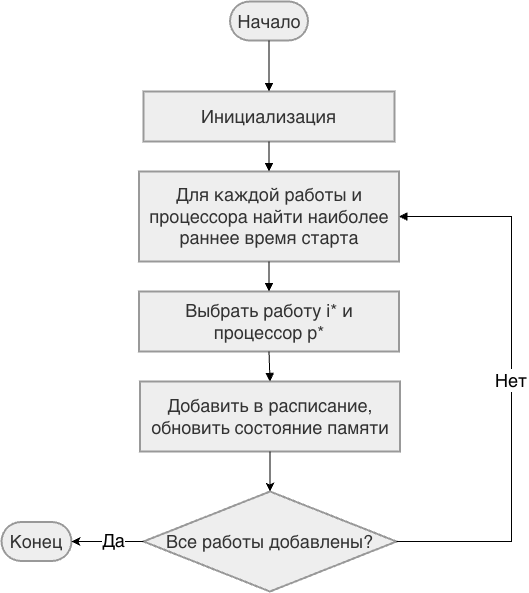
\includegraphics[width=0.63\textwidth]{pictures/gred3.png}
	\captionof{figure}{Блок-схема ЖА}
	\label{fig:gred_sch}
\end{center}

\subsection{Эвристики выбора работы}
\label{subsec:heuristics}

Ключевым элементом жадного алгоритма является правило выбора работы из множества готовых. В данной работе рассматриваются две эвристики: \textbf{EFT} (Earliest Finish Time) и \textbf{STS} (Smallest Time-Space).

\subsubsection*{Эвристика EFT}

Эвристика EFT ориентирована на минимизацию времени завершения работы. После того как для каждой готовой работы $i$ и каждого процессора $p$ определено наиболее раннее допустимое время старта $t_{i,p}$, вычисляется время завершения:
\[
f_{i,p} = t_{i,p} + d_i.
\]
Затем выбирается пара $(i^*, p^*)$, дающая наименьшее $f_{i,p}$. В случае равенства предпочтение отдается работе с наименьшим номером (или процессору с наименьшим номером, если несколько процессоров дают одинаковое время завершения для одной работы). Эта эвристика отличается простотой вычисления, но никак не учитывает использование памяти выбираемой работой.

\subsubsection*{Эвристика STS}

Эвристика STS введена для учёта влияния работы на использование памяти в будущем. Оценка работы складывается из двух компонент.

Первая компонента учитывает собственные буферы работы:
\[
S^{(1)}_i = d_i \cdot \sum_{j=1}^{n_i} r_{ij}.
\]
То есть произведение длительности работы на суммарный объём создаваемых ею буферов.

Вторая компонента учитывает «нагрузку» на память, создаваемую потомками работы. Для каждого буфера $j$ работы $i$ определим множество его потребителей $\mathit{Cons}(i,j) = \{ k \mid (i,k,j) \in E \}$. Пусть $d_{\mathit{total}}(i,j)$ — суммарная длительность всех работ-потребителей этого буфера (каждый потребитель учитывается один раз, даже если он использует несколько буферов). Тогда
\[
S^{(2)}_i = \sum_{j=1}^{n_i} \left( r_{ij} \cdot \sum_{k \in \mathit{Cons}(i,j)} d_k \right).
\]

Общая оценка работы $i$ равна
\[
\phi(i) = S^{(1)}_i + S^{(2)}_i.
\]

Алгоритм выбирает работу с наименьшим значением $\phi(i)$. Если несколько работ имеют одинаковую оценку, то среди них выбирается работа с наименьшим временем завершения (т.е. срабатывает правило EFT). Идея эвристики STS заключается в том, что работа, которая создаёт большие буферы и эти буферы нужны долго выполняющимся потомкам, потребляет память на длительное время, поэтому её выгодно выполнить позже (чтобы не блокировать память). Соответственно, на ранних шагах следует выбирать работы с малым $\phi(i)$.
